\chapter{Ten Puzzle Solver Result}

Paikin~\& Tal \cite{paikin2015} showed the results solving a maximum of five puzzles; what is more, they also provided the solver with the number of input puzzles.  The Mixed-Bag Solver has shown that it can assemble up to 10 puzzles with results comparable to the Paikin~\& Tal solver on each image individually.

Figures~\ref{fig:firstSet10PuzzleInputImages} and~\ref{fig:secondSet10PuzzleInputImages} show the input images supplied to both the Mixed-Bag and Paikin~\& Tal solvers. The 5,850 pieces come from images that are five different sizes.

\begin{figure}
\centering
  \begin{tabular}{ >{\centering\arraybackslash}m{0.45\textwidth} >{\centering\arraybackslash}m{0.45\textwidth} }

	\fbox{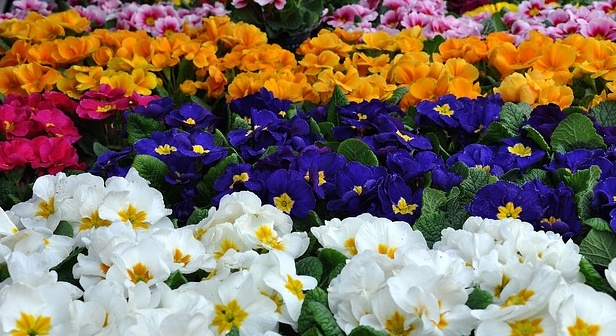
\includegraphics[scale=0.2]{./images/10_puzzles/primula_pixabay.jpg}} & \fbox{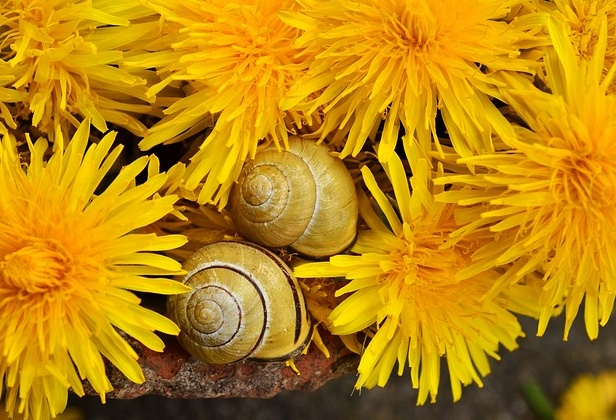
\includegraphics[scale=0.2]{./images/10_puzzles/dandelion_pixabay.jpg}} \\~\\
	(a) 264 Pieces \cite{pixabay} & (b) 330 Pieces \cite{pixabay}
\\~\\
	\fbox{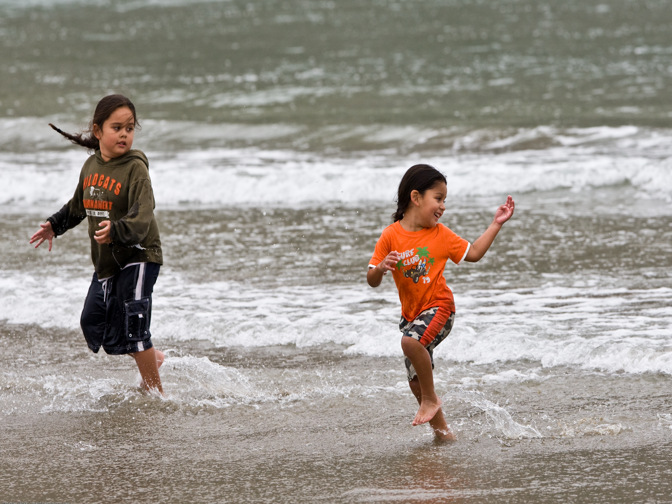
\includegraphics[scale=0.2]{./images/10_puzzles/cho_432_18.png}} & \fbox{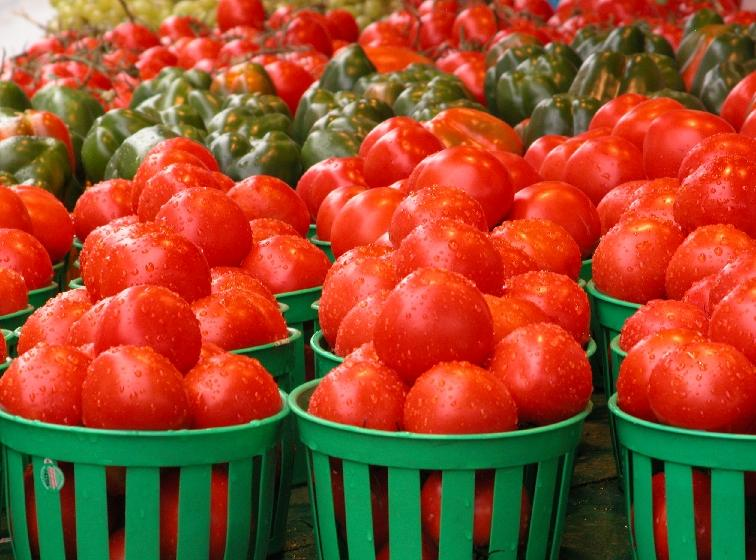
\includegraphics[scale=0.2]{./images/10_puzzles/mcgill_540_16.jpg}} \\~\\
	(c) 432 Pieces \cite{cho2010} & (d) 540 Pieces \cite{pomeranzBenchmarkImages} 
\\~\\
	\fbox{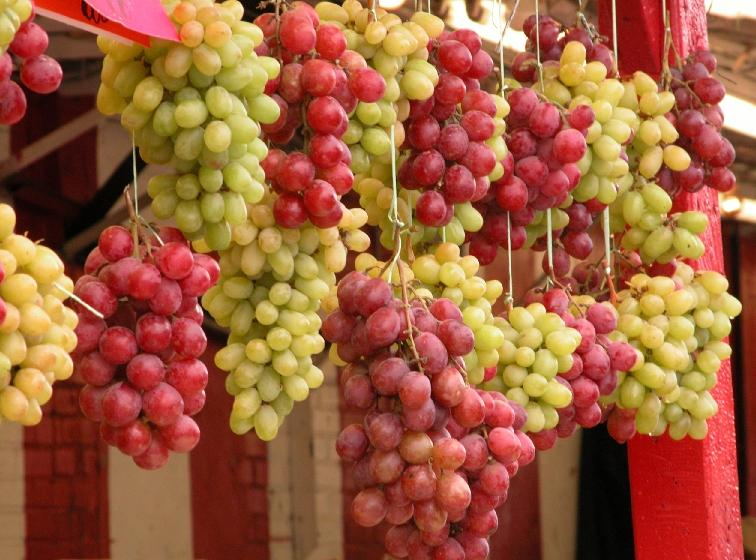
\includegraphics[scale=0.2]{./images/10_puzzles/mcgill_540_15.jpg}} & \fbox{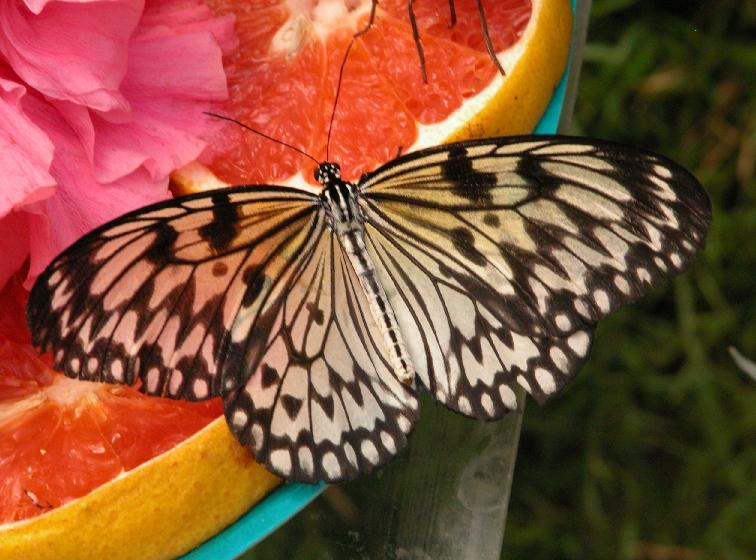
\includegraphics[scale=0.2]{./images/10_puzzles/mcgill_540_7.jpg}}
\\~\\
	(e) 540 Pieces \cite{pomeranzBenchmarkImages} & (f) 540 Pieces \cite{pomeranzBenchmarkImages}
  \end{tabular}

\caption{First Set of Six Images Comprising the 10 Image Test Set}
\label{fig:firstSet10PuzzleInputImages}
\end{figure}

\begin{figure}
\centering
  \begin{tabular}{ >{\centering\arraybackslash}m{0.5\textwidth} >{\centering\arraybackslash}m{0.5\textwidth} }

	\fbox{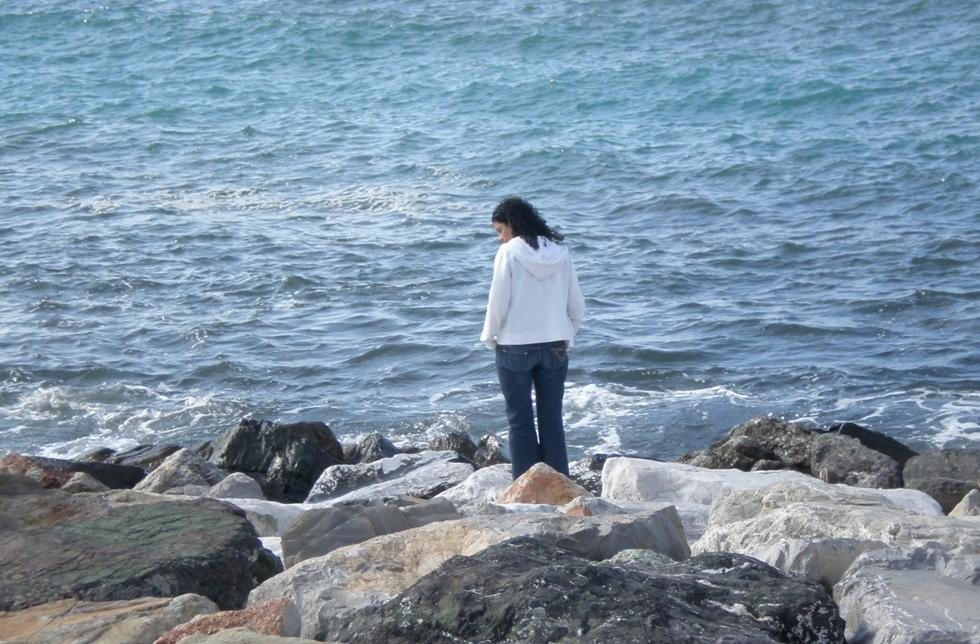
\includegraphics[scale=0.2]{./images/10_puzzles/pomeranz_805_8.jpg}} & \fbox{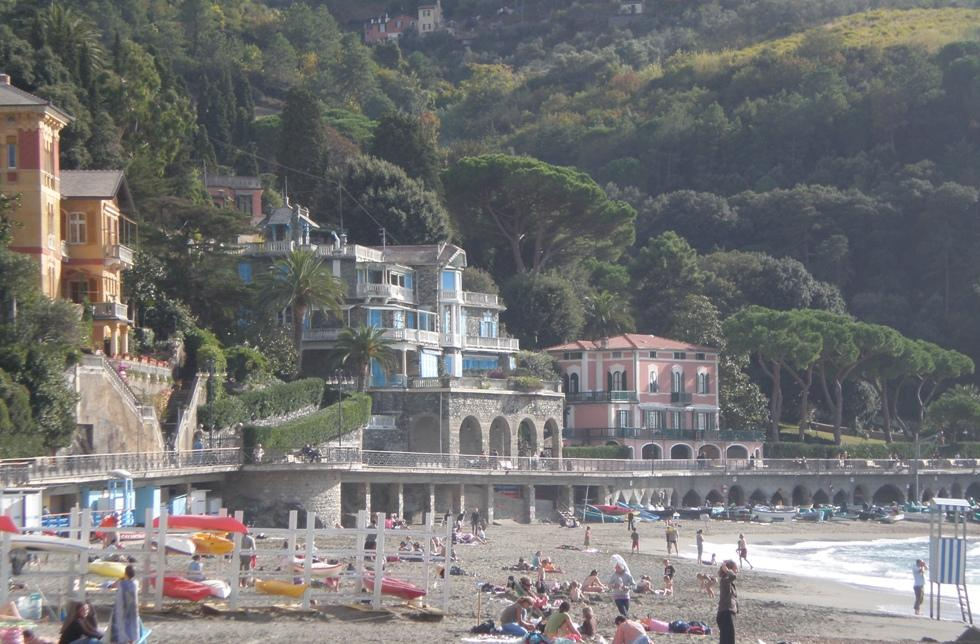
\includegraphics[scale=0.2]{./images/10_puzzles/pomeranz_805_13.jpg}} \\~\\
	(g) 805 Pieces \cite{pomeranzBenchmarkImages} & (h) 805 Pieces \cite{pomeranzBenchmarkImages} 
\\~\\
	\fbox{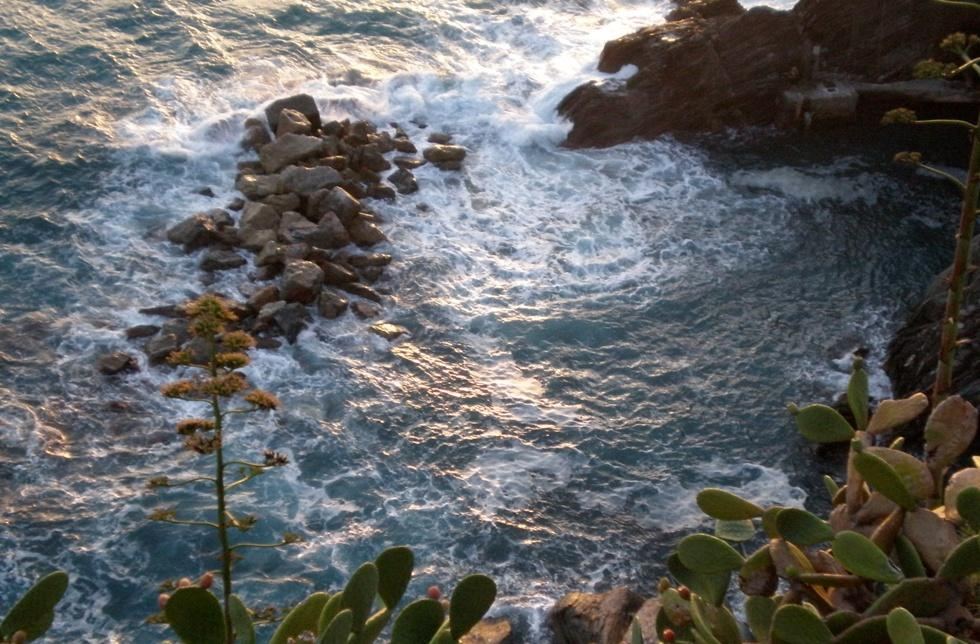
\includegraphics[scale=0.2]{./images/10_puzzles/pomeranz_805_14.jpg}} & \fbox{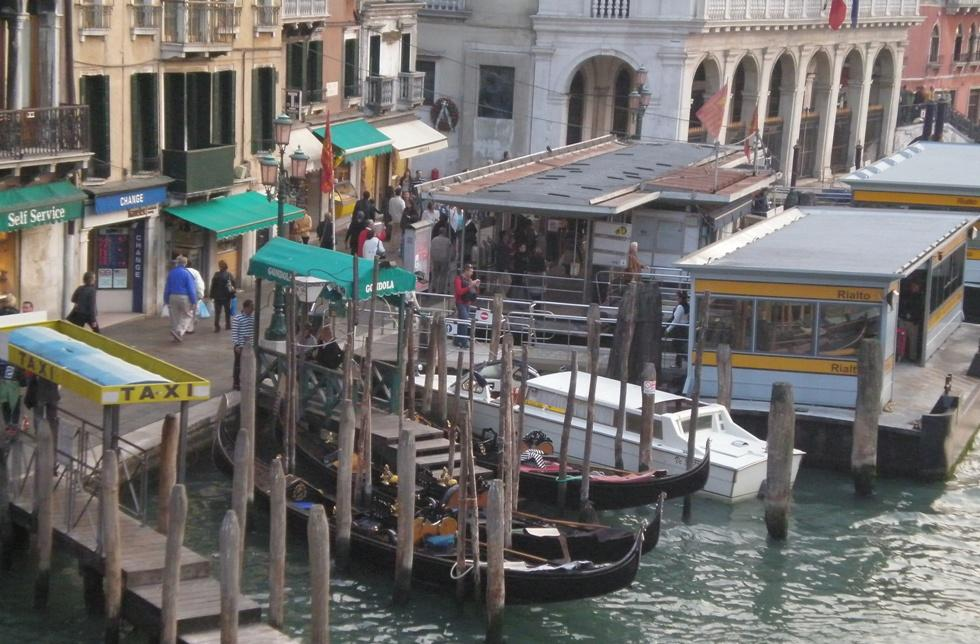
\includegraphics[scale=0.2]{./images/10_puzzles/pomeranz_805_19.jpg}}
\\~\\
	(i) 805 Pieces \cite{pomeranzBenchmarkImages} & (j) 805 Pieces \cite{pomeranzBenchmarkImages}
  \end{tabular}

\caption{Second Set of Four Images Comprising the 10 Image Test Set}
\label{fig:secondSet10PuzzleInputImages}
\end{figure}
